%%% Xi'an Jiaotong University presentation beamer template
%%% modified from UU_beamer v2.0 by King-Siong Si, Institute of Multimedia Knowledge Fusion and Engineering, Xi'an JiaoTong University

\documentclass{beamer}

\usepackage{ctex}
\usepackage[english]{babel} % comment this line and use the next one if you want a chinese style
% \usepackage[chinese, provide=*]{babel}
\usepackage[utf8x]{inputenc}
\usepackage{hyperref, % clickable links
    graphicx, % include images
    listings, % for code and formatting
    caption, % customization of captions in figures and tables
    stackengine, % custom layouts 
    amsmath, % math env
    xcolor, % extend color support
    multicol, % multiple columns layout
    multirow, % multiple rows layout
    booktabs, % high quality tables
    tikz, % tikz for drawing
    pgfplots, % pgfplots for drawing functions
    bm
}
\usetikzlibrary{calc, shapes.symbols}

% ------ FONT STYLES ------ %

\setCJKfamilyfont{oyx-tc}{AuIongSun-TC.TTC}[Path=./fonts/]
\setCJKfamilyfont{oyx-sc}{AuIongSun-SC.otf}[Path=./fonts/]
\newcommand{\oyxtc}{\CJKfamily{oyx-tc}}
\newcommand{\oyxsc}{\CJKfamily{oyx-sc}}

\setCJKsansfont[Path=./fonts/]{AuIongSun-TC.TTC} % traditional chinese
% \setCJKsansfont[Path=./fonts/]{AuIongSun-SC.otf} % simplified chinese

\usepackage{xjtu_beamer} % customized style

% ------ COMMANDS ------ %

\def\cmd#1{\texttt{\color{red}\footnotesize $\backslash$#1}}
\def\env#1{\texttt{\color{blue}\footnotesize #1}}

\newcommand{\hl}[1]{\textcolor{uppsalared}{#1}} % highlight
%%% to avoid footnote rule from showing too early when using overalys. 
%%% ugly, but it works. 
%%% this method comes from https://tex.stackexchange.com/questions/518750/beamer-how-to-make-footnote-rule-appear-later-pause.
\newcommand{\onlyfootnoterule}[1]{\let\oldfootnoterule\footnoterule
\def\footnoterule{\only<#1>{\oldfootnoterule}}}
\newcommand{\uncoverfootnoterule}[1]{\let\oldfootnoterule\footnoterule
\def\footnoterule{\uncover<#1>{\oldfootnoterule}}}

% ------ CODE COLOR DEFINITION ------ %

\definecolor{codered}{rgb}{0.6,0,0}
\definecolor{codeblue}{rgb}{0,0,0.8}
\definecolor{codegreen}{rgb}{0,0.5,0}
\definecolor{almostwhite}{gray}{0.55}
\definecolor{codepurple}{rgb}{0.58,0,0.82}
\definecolor{backcolour}{rgb}{0.95,0.95,0.92}

\lstset{
    basicstyle=\ttfamily\small,
    keywordstyle=\bfseries\color{codeblue},
    emphstyle=\ttfamily\color{codered},   % Custom highlighting style
    stringstyle=\color{codepurple},
    numbers=left,
    numberstyle=\small\color{almostwhite},
    rulesepcolor=\color{red!20!green!20!blue!20},
    frame=shadowbox,
    commentstyle=\color{codegreen},
    captionpos=b    
}

% ------ PRESENTATION INFO ------ %
\newcommand{\fullconference}{Conference Name} % used for conference
\newcommand{\shortconference}{Conference acronym}
\newcommand{\contact}
{\href{mailto:sjsinx@stu.xjtu.edu.cn}{\textit{sjsinx@stu.xjtu.edu.cn}}}

\author[K. Si, \contact]{\href{}{King-Siong Si}}
\institute[IMKFE, XJTU]{\href{}{Institute of Multimedia Knowledge Fusion and Engineering,\\ Xi'an JiaoTong University}
    \\ \smallskip \contact}
\title[beamer]{how to make a presentation}
% \subtitle{subtitle}
\date{\today}

\begin{document}

% ------ TITLE SLIDE ------ %
{
% Remove headline and footline from first slide
\setbeamertemplate{footline}{} 
\setbeamertemplate{headline}{} 
\setbeamertemplate{navigation symbols}{}

\begin{frame}\label{start}
    \titlepage
    \begin{figure}
            
\includegraphics[width=.2\textwidth]{style/xjtu_logo.png} 
    \end{figure}
\end{frame}
}

% ------ TABLE OF CONTENT ------ %
\begin{frame}
    \tableofcontents[sectionstyle=show, subsectionstyle=show/shaded/hide, subsubsectionstyle=show/shaded/hide]
\end{frame}

% ------ MAIN BODY ------ %

\section{Introduction}

{
\uncoverfootnoterule{2-} % control the showing time of footnote rule
\begin{frame}{Example of text and equation}

    a beamer template modified from \href{https://www.overleaf.com/latex/templates/uppsala-university-beamer-template-v2-dot-0/sjbwbmzvpbbf}{Uppsala University presentation beamer template}.

    this is a citation.\cite{vaswani2017attention}
    this is a piece of \hl{highlighted text}.

    \begin{itemize}[<+->] % overlay
        \item 1st, we should sleep more...
        \item 2nd, we should eat more...\footnote<2->{this is a footnote.}
    \end{itemize}

    \begin{block}{Block Title}
        Block 1
    \end{block}

    \centering
    \begin{equation}
        x = \frac{{-a \pm \sqrt{{b}}}}{{c}}
        \label{eq:equation1}
    \end{equation}

    In Equation~\ref{eq:equation1}, we have the \textit{bla bla bla} formula.

\end{frame}
}

\section{Methodology}
\begin{frame}{Two columns layout}
    % ------ TWO COLUMNS LAYOUT ------ %
    \begin{columns}

        \column{0.5\textwidth}
        \begin{itemize}
            \item Item 1
            \item Item 2 
            \begin{itemize}
                \item Subitem 
            \end{itemize}
        \end{itemize}
        
        \column{0.5\textwidth}
        \begin{figure}
            \centering
            
\includegraphics[height=0.5\textwidth]{images/placeholder_image.png}
            \caption{Image caption}
            \label{fig:figure1}
        \end{figure}
        
    \end{columns}

    
\end{frame}

\begin{frame}{Code snippet example}
    \lstinputlisting[language=Python, label=samplecode, caption=Example of code, % firstline=1, lastline=10
    ]{code.py}
\end{frame}

\begin{frame}[t]{TikZ overlay example} % awful example since i'm rubbish
    \begin{itemize}[<+->]
        \item \textit{RepVGG: Making VGG-style ConvNets Great Again}\cite{ding2021repvgg}
    \end{itemize}
    \uncover<2->{
        \begin{figure}
            \centering
            \resizebox{.6\textwidth}{!}{
                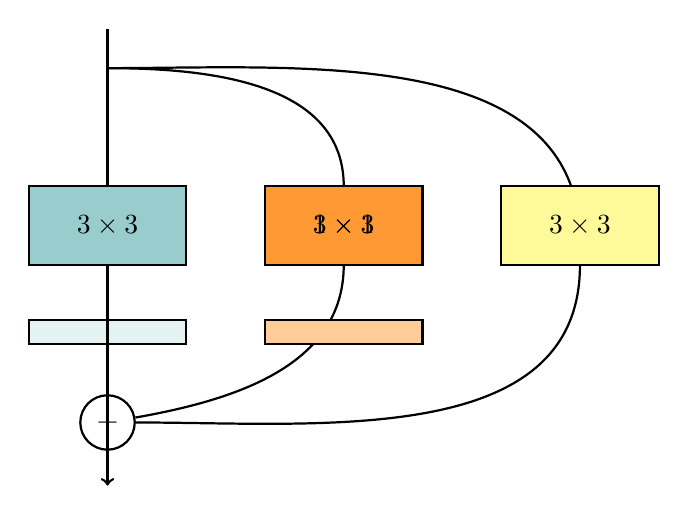
\begin{tikzpicture}
                    % \draw [help lines] (0, 0) grid (10, 10);
                    \draw [thick, fill=teal!40] (0, 5) rectangle (2, 6);
                    \uncover<2-3>{
                    \draw [thick, fill=orange!80] (3, 5) rectangle (5, 6);}
                    \uncover<2>{
                    \draw [thick, fill=yellow!40] (6, 5) rectangle (8, 5.3);}
                    
                    \draw [thick] (1, 8) -- (1, 6);
                    \uncover<2-3>{
                    \draw [thick] (1, 7.5) to [out=0, in=90] (4, 6);
                    \draw [thick, out=0, in=90] (1, 7.5) to (7, 5.3);}
                    
                    \uncover<2-3>{
                    \node (add) [circle, minimum size=1, thick, draw=black] at (1, 3) {\textbf{$+$}};}
                    \uncover<2-3>{
                    \draw [thick] (1, 5) -- (add);}
                    \uncover<2-3>{
                    \draw [thick, out=270, in=10] (4, 5) to (add);
                    \draw [thick, out=270, in=0] (7, 5) to (add);}
                
                    \uncover<2>{
                    \draw [thick, fill=teal!10] (0, 4) rectangle (2, 4.3);
                    \draw [thick, fill=orange!40] (3, 4) rectangle (5, 4.3);}
                    \uncover<2-3>{
                    \draw [thick, ->] (add) -- (1, 2.2);}
                    \uncover<4>{
                        \draw [thick, ->] (1, 5) -- (1, 2.2);
                    }
                
                    \node (dot1) at (1, 5.5) {$3\times 3$};
                    \uncover<2>{
                    \node (dot2) at (4, 5.5) {$1\times 1$};}
    
                    \uncover<3>{
                    \draw [thick, fill=yellow!40] (6, 5) rectangle (8, 6);}
    
                    \uncover<3>{
                    \node (dot2) at (4, 5.5) {$3\times 3$};
                    \node (dot3) at (7, 5.5) {$3\times 3$};}
                
                \end{tikzpicture}
            }
        \end{figure}
    }
\end{frame}


\begin{frame}{Table frame example}

\begin{table}
    \begin{tabular}{c|cc}
        \textbf{Col1} & Col2 & Col3 \\
        \hline
        1            & ...                    & ...             \\
        2            & ...                    & ...             \\
        3            & ...                    & ...             \\
    \end{tabular}
    \caption{Table name}
    \label{tab:table1}
\end{table}

\end{frame}

\begin{frame}{中文正體測試}
    \begin{itemize}
        \item 此字體為歐體風格,源於著名碑帖《九成宮醴泉銘》。
        \item 大決所犯,傷人必多,吾不克救也。---《春秋左傳》
        \item 帝高陽之苗裔兮,朕皇考曰伯庸。---《離騷經》
        \item 溥天之下,莫非王土;率土之濱,莫非王臣。---《詩經》
        \item 歸去來兮,請息交以絕遊。---《歸去來辭並序》
        \item 後之視今,亦由今之視昔。---《蘭亭集序》
        \item 天地玄黃,宇宙洪荒。---《千字文》
        \item 欲買桂花同載酒,終不似,少年遊。---《唐多令》
        \item 昨夜西風凋碧樹,獨上高樓,望盡天涯路。---《蝶戀花》
        \item 衣帶漸寬終不悔,為伊消得人憔悴。---《鳳棲梧》
        \item 暮然回首,那人卻在燈火闌珊處。---《青玉案》
        \item 精勤求學,敦篤勵志,果毅力行,忠恕任事。\\---西安交通大學校訓
        \item 嚴、正、勤、實。---養正中學校訓
    \end{itemize}
\end{frame}

{
    \oyxsc
    \begin{frame}{\oyxsc 中文简体测试}
        \begin{itemize}
            \item 此字体为欧体风格,源于著名碑帖《九成宫醴泉铭》。
            \item 大决所犯,伤人必多,吾不克救也。---《春秋左传》
            \item 帝高阳之苗裔兮,朕皇考曰伯庸。---《离骚经》
            \item 溥天之下,莫非王土;率土之滨,莫非王臣。---《诗经》
            \item 归去来兮,请息交以绝游。---《归去来辞并序》
            \item 后之视今,亦由今之视昔。---《兰亭集序》
            \item 天地玄黄,宇宙洪荒。---《千字文》
            \item 欲买桂花同载酒,终不似,少年游。---《唐多令》
            \item 昨夜西风凋碧树,独上高楼,望尽天涯路。---《蝶恋花》
            \item 衣带渐宽终不悔,为伊消得人憔悴。---《凤栖梧》
            \item 暮然回首,那人却在灯火阑珊处。---《青玉案》
            \item 精勤求学,敦笃励志,果毅力行,忠恕任事。\\---西安交通大学校训
            \item 严、正、勤、实。---养正中学校训
        \end{itemize}
    \end{frame}
}

\section{Conclusion}

\begin{frame}{Conclusion}
    \begin{itemize}
        \item sleep is all we need.
    \end{itemize}
    \begin{figure}
        \centering
        
\includegraphics[height=5cm]{images/placeholder_image.png}
        \caption{Image caption}
        \label{fig:figure2}
    \end{figure}
\end{frame}

% ------ REFERENCES ------ %

\section{References}

\begin{frame}[allowframebreaks] % auto break frames
    \bibliography{ref}
    \tiny\bibliographystyle{plain}
\end{frame}

\section*{Thanks}

{
% use Le-Su motto in the last slide
\usebackgroundtemplate{
    \begin{tikzpicture}[overlay,remember picture]
        % Background picture
        \node[at=(current page.center),anchor=center, inner sep=0pt,outer sep=0pt, fill opacity=.3] {
            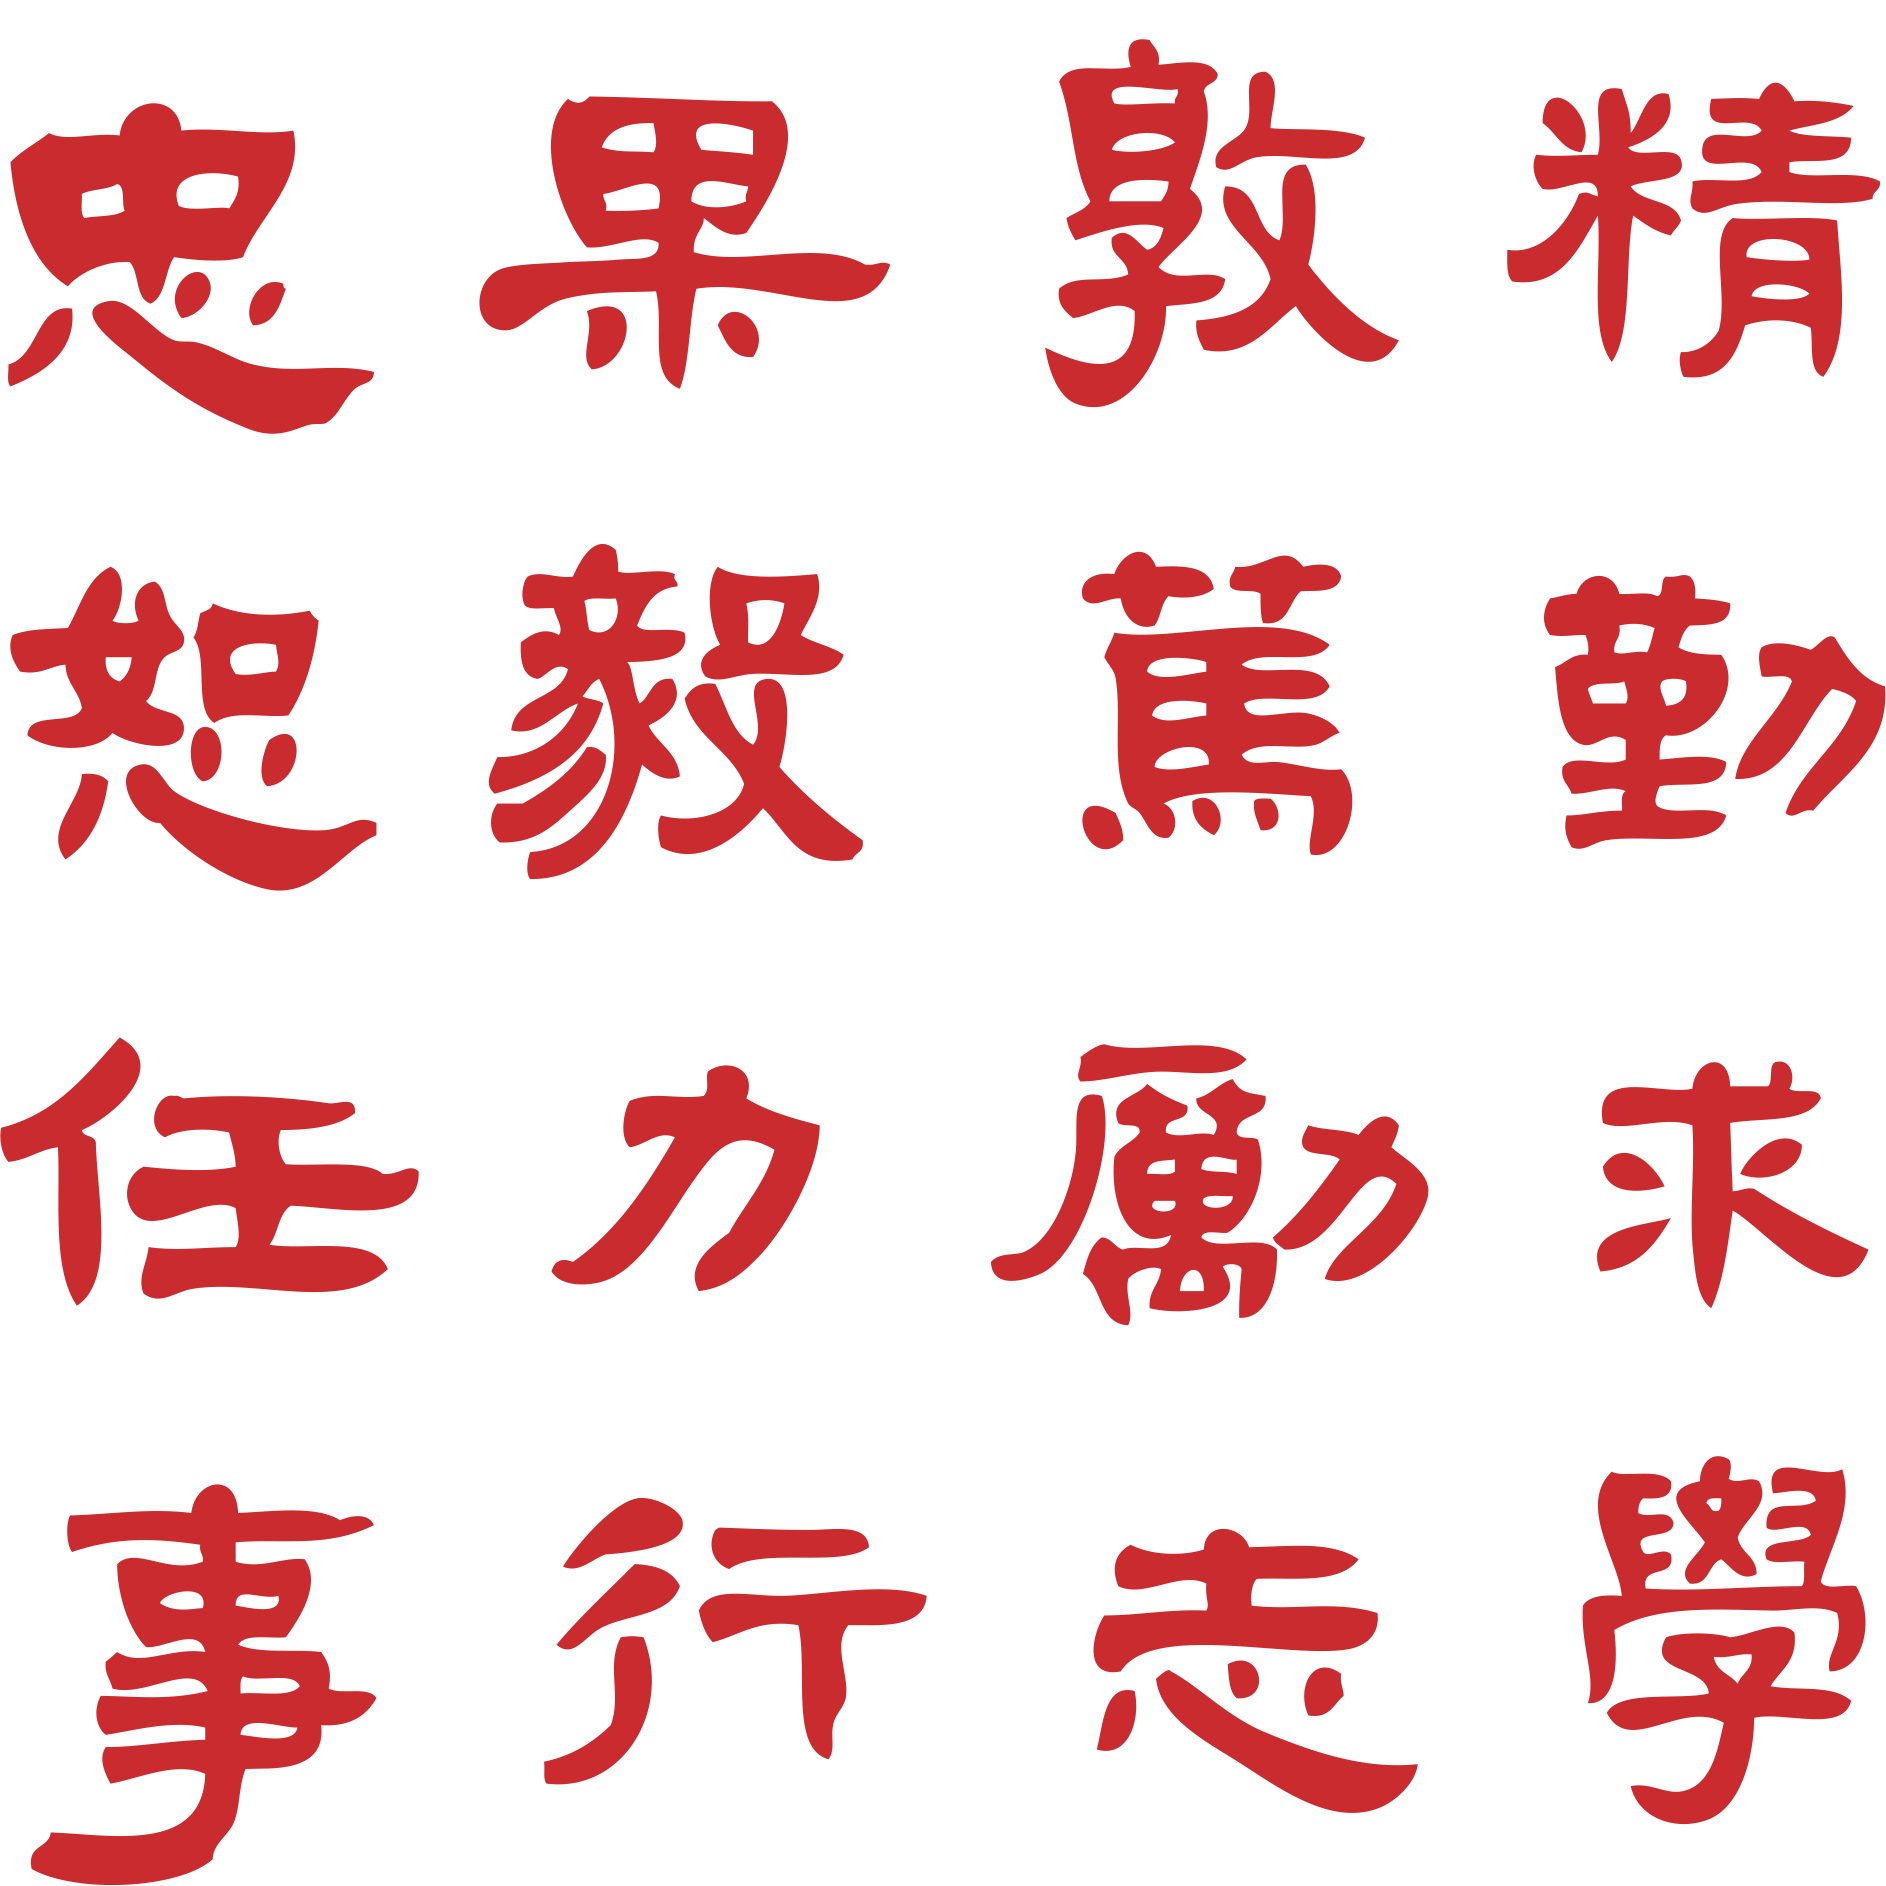
\includegraphics[keepaspectratio,height=.8\paperheight]{style/xjtu_motto_origin.png}};
    \end{tikzpicture}
}
    
\begin{frame}
    \begin{tikzpicture}[overlay,remember picture]
        % make it in center position
        \node[at=(current page.center),anchor=center,inner sep=0pt,outer sep=0pt] 
        {\Huge \textsc{Thanks!}};
    \end{tikzpicture}
\end{frame}
}

\end{document}
